\documentclass[tikz,border=9pt]{standalone}
\usepackage{amsmath,amssymb}
\usetikzlibrary{arrows.meta,positioning,calc}
\begin{document}
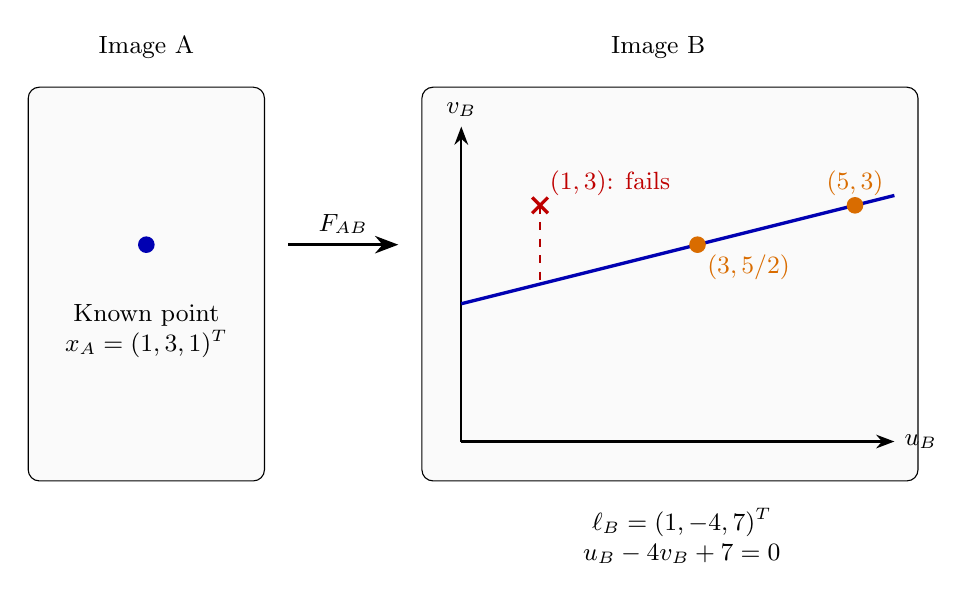
\begin{tikzpicture}[font=\small,arr/.style={-{Stealth},thick},box/.style={draw=blue!55!black,rounded corners,fill=blue!4,align=center,text width=2.9cm,minimum height=1.05cm}]

\draw[rounded corners,fill=gray!4] (-3,-.5) rectangle (0,4.5);
\node at (-1.5,5){Image A};
\fill[blue!70!black] (-1.5,2.5) circle(3pt);
\node[align=center] at (-1.5,1.4){Known point\\$x_A=(1,3,1)^T$};
\draw[arr,very thick] (.3,2.5)--(1.7,2.5) node[midway,above]{$F_{AB}$};
\node at (5,5){Image B};
\draw[rounded corners,fill=gray!4] (2,-.5) rectangle (8.3,4.5);
\draw[arr] (2.5,0)--(8,0) node[right]{$u_B$};
\draw[arr] (2.5,0)--(2.5,4) node[above]{$v_B$};
\draw[very thick,blue!70!black] (2.5,1.75)--(8,3.125);
\fill[orange!85!black] (5.5,2.5) circle(3pt) node[below right]{$(3,5/2)$};
\fill[orange!85!black] (7.5,3) circle(3pt) node[above]{$(5,3)$};
\draw[red!75!black,very thick] (3.4,2.9)--(3.6,3.1) (3.4,3.1)--(3.6,2.9);
\node[above right,red!75!black] at (3.5,3){$(1,3)$: fails};
\draw[dashed,red!70!black] (3.5,3)--(3.5,2);
\node[align=center] at (5.3,-1.2){$\ell_B=(1,-4,7)^T$\\$u_B-4v_B+7=0$};

\end{tikzpicture}
\end{document}
